%==========================================================================
%Template File for Monthly Lectual Meeting
%2006/05/22 (kkobayashi@mikilab.doshisha.ac.jp)
%==========================================================================
\documentclass[a4j,9pt,twocolumn]{jsarticle}
\usepackage{mlm2.0}
\usepackage{epsf}
\pagestyle{plain}
\usepackage{url}
\usepackage{subfigure}
\setcounter{page}{1}
\usepackage{geometry}
\geometry{left=25mm,right=25mm,top=20mm,bottom=30mm}
%\usepackage[dvips]{graphicx}

\begin{document}
\twocolumn[
%---------------------------------------------------------------------------        % ヘッダ    書式:\beginheader{回}{年}{月}
%---------------------------------------------------------------------------
\beginheader{170}{2016}{04}
%---------------------------------------------------------------------------
% 発表題目    書式:\title{日本語}{英語} 「\\」で改行できます
%---------------------------------------------------------------------------
\title%
{git}%
%{更なる大容量化を目指して 進化しつづける次世代光メディア}

%---------------------------------------------------------------------------
% 著者名      書式:\author{日本語著者名}{英語著者名}
%---------------------------------------------------------------------------
\author{山下 俊樹,外村 篤紀\\Toshiki YAMASHITA,Atsuki TONOMURA}

%---------------------------------------------------------------------------
\endheader
%\begin{abstract}
%---------------------------------------------------------------------------
%Recently, a DVD attracts attention along with the image and the digitization of the sound. The standards of these DVD are complicated. So, in this paper, the standards of the DVD are summarized and the DVD of the next generation is refered. 
%---------------------------------------------------------------------------
%\end{abstract}
]

%---------------------------------------------------------------------------
% 本文
%---------------------------------------------------------------------------

\section{はじめに}
近年,ソフトウエアは大規模化し,修正を行う対象の数が増加したため,その更新頻度は増加の一途を辿っている.そこで,コンピューター上で作成,および編集されるファイルの変更履歴を管理するバージョン管理システムの重要性が増している.バージョン管理システムには,管理下のファイルを任意の記録時点の状態に復元することができる,および一つのファイルを複数人で編集する場合,競合が発生しないように管理が行われるなどの利点があるため,注目を集めている\cite{pop}.

バージョン管理システムには,サーバ上のみでファイルの管理を行う集中型バージョン管理システムと,サーバに加え,個人のPCでも管理を行う分散型バージョン管理システムがある.本報告では,分散型バージョン管理システムの一つであるgitの概要,内部構造,および利点について述べる.

\section{git}
\subsection{gitの構成}
gitの構成を以下の\fgref{git}に示す.

\begin{figure}[h]
\centering
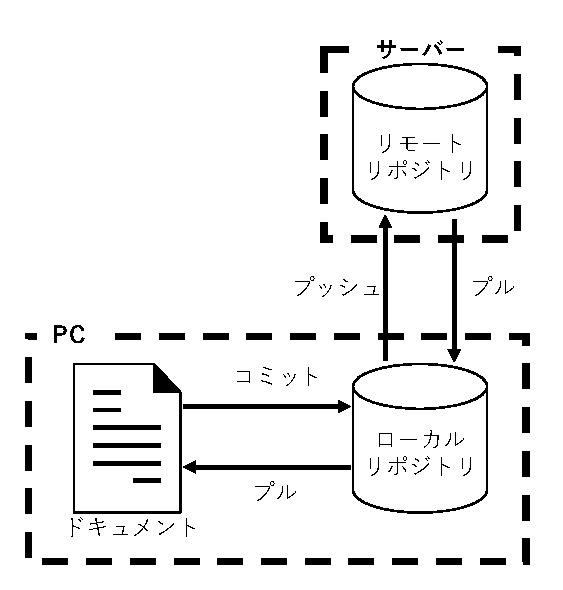
\includegraphics[width=70mm]{img/git.eps}
\caption{gitの構成}
\label{git}
\end{figure}

gitで管理されるファイルやディレクトリの変更内容は,リポジトリと呼ばれる一種のデータベースに蓄積される.分散型バージョン管理システムにおけるリポジトリは,サーバ上に配置され,複数ユーザで利用するリモートリポジトリと,個人のPC内に配置され,その個人が利用するローカルリポジトリに分類される.ユーザがファイルやディレクトリの変更をローカルリポジトリに記録する操作をコミットと呼び,これを実行すると最新の状態が記録される.過去のコミット時点の状態への復元操作,およびブランチを切り替える操作をチェックアウトと呼ぶ.コミットやプッシュを行うことで作業成果を記録し,プルを行うことでリモートリポジトリから他者の作業成果をダウンロードして統合することができる.

\subsection{ブランチ}
\subsubsection{概要}
gitの特徴の一つであるブランチについて述べる.ブランチの概念図を以下の\fgref{branch}に示す.

\begin{figure}[h]
\centering
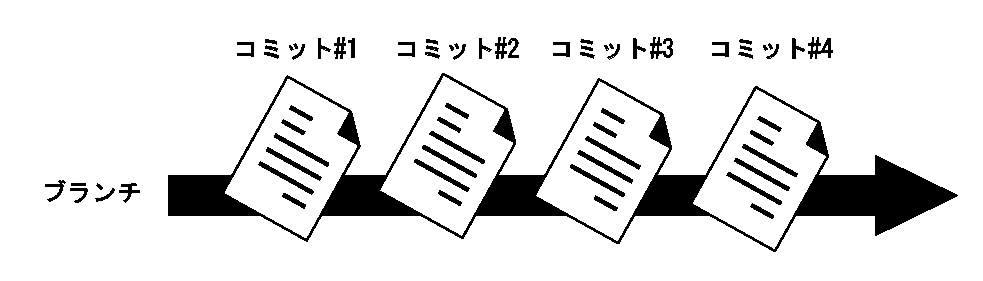
\includegraphics[width=75mm]{img/branch1.eps}
\caption{ブランチの概念}
\label{branch}
\end{figure}

ブランチとは,蓄積されたコミットの時系列と,系列を分岐する操作を指す.分岐したブランチ同士は互いに独立しており,任意のブランチ内のコミットは他のブランチでのコミットの影響を受けない.ブランチ同士の結合はマージと呼ぶ.

\subsubsection{バグ修正におけるブランチの有用性}
ブランチを利用した一例を以下の\fgref{branch_ex}に示す.

\begin{figure}[h]
\centering
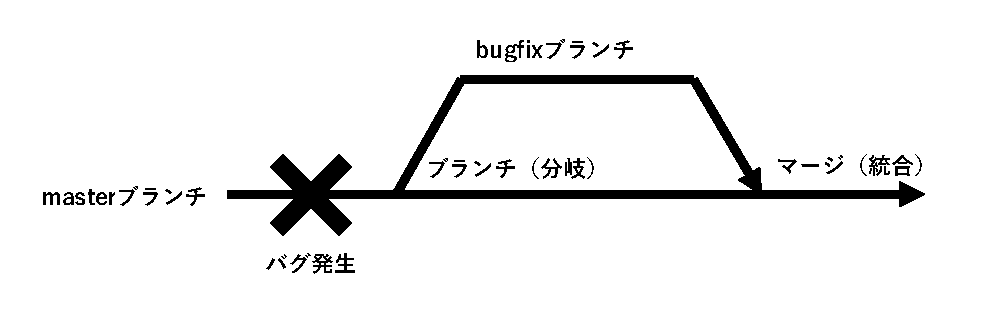
\includegraphics[width=80mm]{img/branch.eps}
\caption{ブランチの一例}
\label{branch_ex}
\end{figure}

ブランチを用いることで,様々な開発やバグ修正などを同時並行で行うことができる.具体的には,\fgref{branch_ex}において既に運用されているソフトウエアの管理を行っているブランチをmasterブランチとし,そのソフトウエアのバグを修正するために用意したブランチをbugfixブランチとする.この場合,二つのブランチは独立しているため,masterブランチに影響を与えることなくbugfixブランチでバグ修正を行うことができる.すなわち,ブランチを使用しない場合は,バグ修正が完了するまでソフトウエアの運用を停止しなければならないが,ブランチを用いることでソフトウエアの運用を止めることなく,平行してバグ修正を行うことができる.バグ修正が完了した後にマージを行えば,ソフトウエアの運用が行われたまま,マージの時点でバグが修正される.さらにブランチの本数を増やせば,リリースしたソフトウエアを運用しながら新機能の追加を行い,さらにバグ修正も同時並行で行うといった運用が可能である.

\subsection{内部構造}
本項では,gitがどのようにバージョン管理を行っているかについて述べる\cite{mecha}.gitで管理されているディレクトリの最上層には.gitディレクトリが生成されており,.gitディレクトリがローカルリポジトリの本体である..gitディレクトリの構成を以下の\fgref{object1}に示す.

\begin{figure}[h]
\centering
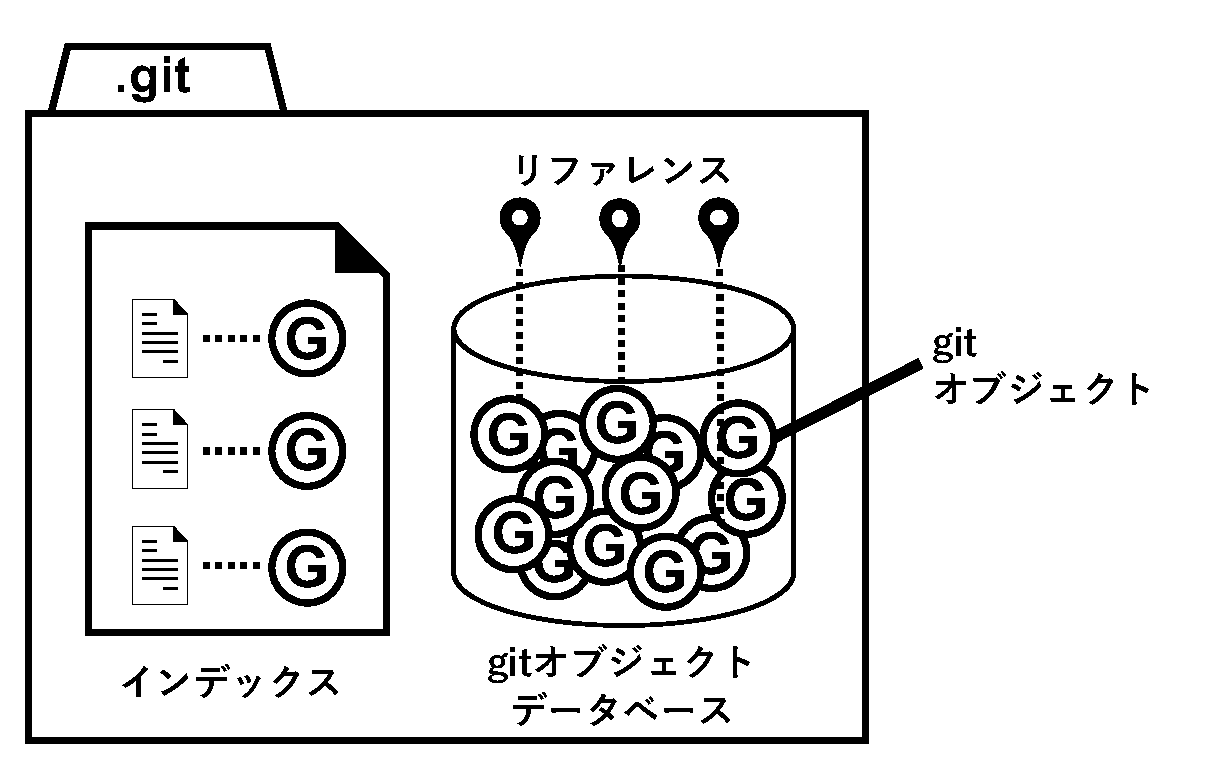
\includegraphics[width=60mm]{img/git_obj.eps}
\caption{.gitディレクトリの構成}
\label{object1}
\end{figure}

.gitディレクトリ内には,gitオブジェクト,リファレンス,およびインデックスが格納されている.gitオブジェクトの集合をgitオブジェクトデータベースと呼ぶ.インデックスはgitオブジェクトのデータベース内の格納位置を示している.gitオブジェクトの内容を以下の\fgref{object2}に示す.

\begin{figure}[h]
\centering
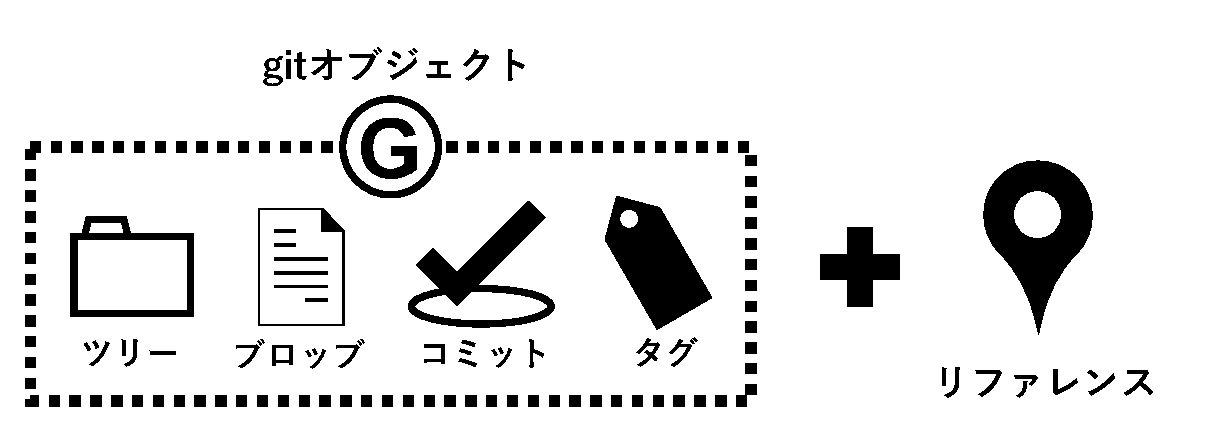
\includegraphics[width=65mm]{img/git_obj2.eps}
\caption{gitオブジェクト}
\label{object2}
\end{figure}

gitオブジェクトは,\fgref{object2}に示す4種類がある.ツリーはディレクトリに,ブロッブはファイルに相当する.gitで管理するディレクトリとファイルをツリーとブロッブに変換し管理する.1つのリファレンスは1つのコミットに対応し,コミットにはツリー,およびブロッブが対応する.リファレンスを用いて,任意のコミットの対象ファイルやディレクトリに芋づる式にアクセスできる.以上のように,コミットごとにディレクトリやファイルがデータベースに蓄積され,リファレンスを付けて管理する.そのため,リファレンスを目次として,過去のいかなるコミットにもアクセスすることができる.過去の状態に戻す場合は,該当時点のリファレンスをたどり,対応するファイルを取り出せばよい.ブランチのように複雑な管理を行う場合でも,リファレンスを用いて管理することにより,処理を軽減し,git全体の動作を高速化している.

\subsection{利点と欠点}
ローカルリポジトリによって,ネットワークに接続されていない環境でもコミットを行うことができる.あるいは,バグ修正のために個人のローカルリポジトリに適量のコミットを行い,修正が完了した後にリモートリポジトリにプッシュし他者に公開するといった使用方法が可能である.

さらに,ブランチ機能が他の他のバージョン管理システムに比べて優れている.他のシステムでは,マージの際にどのファイルをどのようにマージするか明示的に入力する必要があるが,gitは自動的に行う.また,マージにかかる時間も他のシステムに比べて高速である.

欠点は,gitで扱えるファイルの種類がテキストベースのファイルに限られる点である.このため,書類作成のデファクト・スタンダードである,Microsoft Officeで作成したファイルを改変なしでは管理できない.

\section{今後の展望}
今日,ソフトウエアのリリース速度は増加の一途をたどり,その裏では開発の効率化,高速化が重要視されている.そのため,gitのようなバージョン管理ソフトウエアやチケット駆動開発は更に普及すると考えられる.また,現在はGitHubのようなSNSサービスは概ね無料で公開されているが,あるソフトウエアの開発において,デバッグや開発の一部を他者に依頼し,一番良いソースコードを含むフォークに報酬を払うなどのビジネスも近い将来に生まれると考える.

\small
\begin{thebibliography}{99}
\bibitem{pop}
岡本隆史:Gitに潜む光と闇,入手先,(http://gihyo.jp/dev/column/01/prog/2012/git)

\bibitem{mecha}
koseki2:Git の仕組み (1),入手先(http://koseki.\\hatenablog.com/entry/2014/04/22/inside-git-1)
\end{thebibliography}
\end{document}